\section{Exploratory Data Analysis (EDA)}

Quá trình EDA không chỉ dừng lại ở việc quan sát thống kê mô tả, mà còn nhằm mục đích tìm ra các cấu trúc ngầm ẩn, định hướng cho việc lựa chọn mô hình và các kỹ thuật Feature Engineering về sau. Dưới đây là các phân tích chuyên sâu được bóc tách từ tập dữ liệu:

\paragraph{1. Phân phối của biến mục tiêu (\texttt{charges}) và Vấn đề Lệch chuẩn:} 
Hình \ref{fig:dist} cho thấy chi phí y tế có phân phối cực kỳ right-skewed. Hầu hết các quan sát tập trung ở vùng chi phí thấp (quanh mức 5,000 - 10,000 USD), dẫn đến việc mean bị kéo lệch đáng kể so với median. 
Đặc biệt, sự xuất hiện của vùng long tail (những bệnh nhân có chi phí y tế vượt ngưỡng 40,000 USD) tiềm ẩn nguy cơ gây ra hiện tượng Heteroscedasticity khi huấn luyện các mô hình tuyến tính. \textit{Insight} này là cơ sở vững chắc để đề xuất phương pháp Log Transform ở giai đoạn tối ưu hóa, nhằm đưa phân phối biến mục tiêu về dạng tiệm cận chuẩn, giúp các mô hình tính toán khoảng cách hội tụ tốt hơn.

\begin{figure}[H]
    \centering
    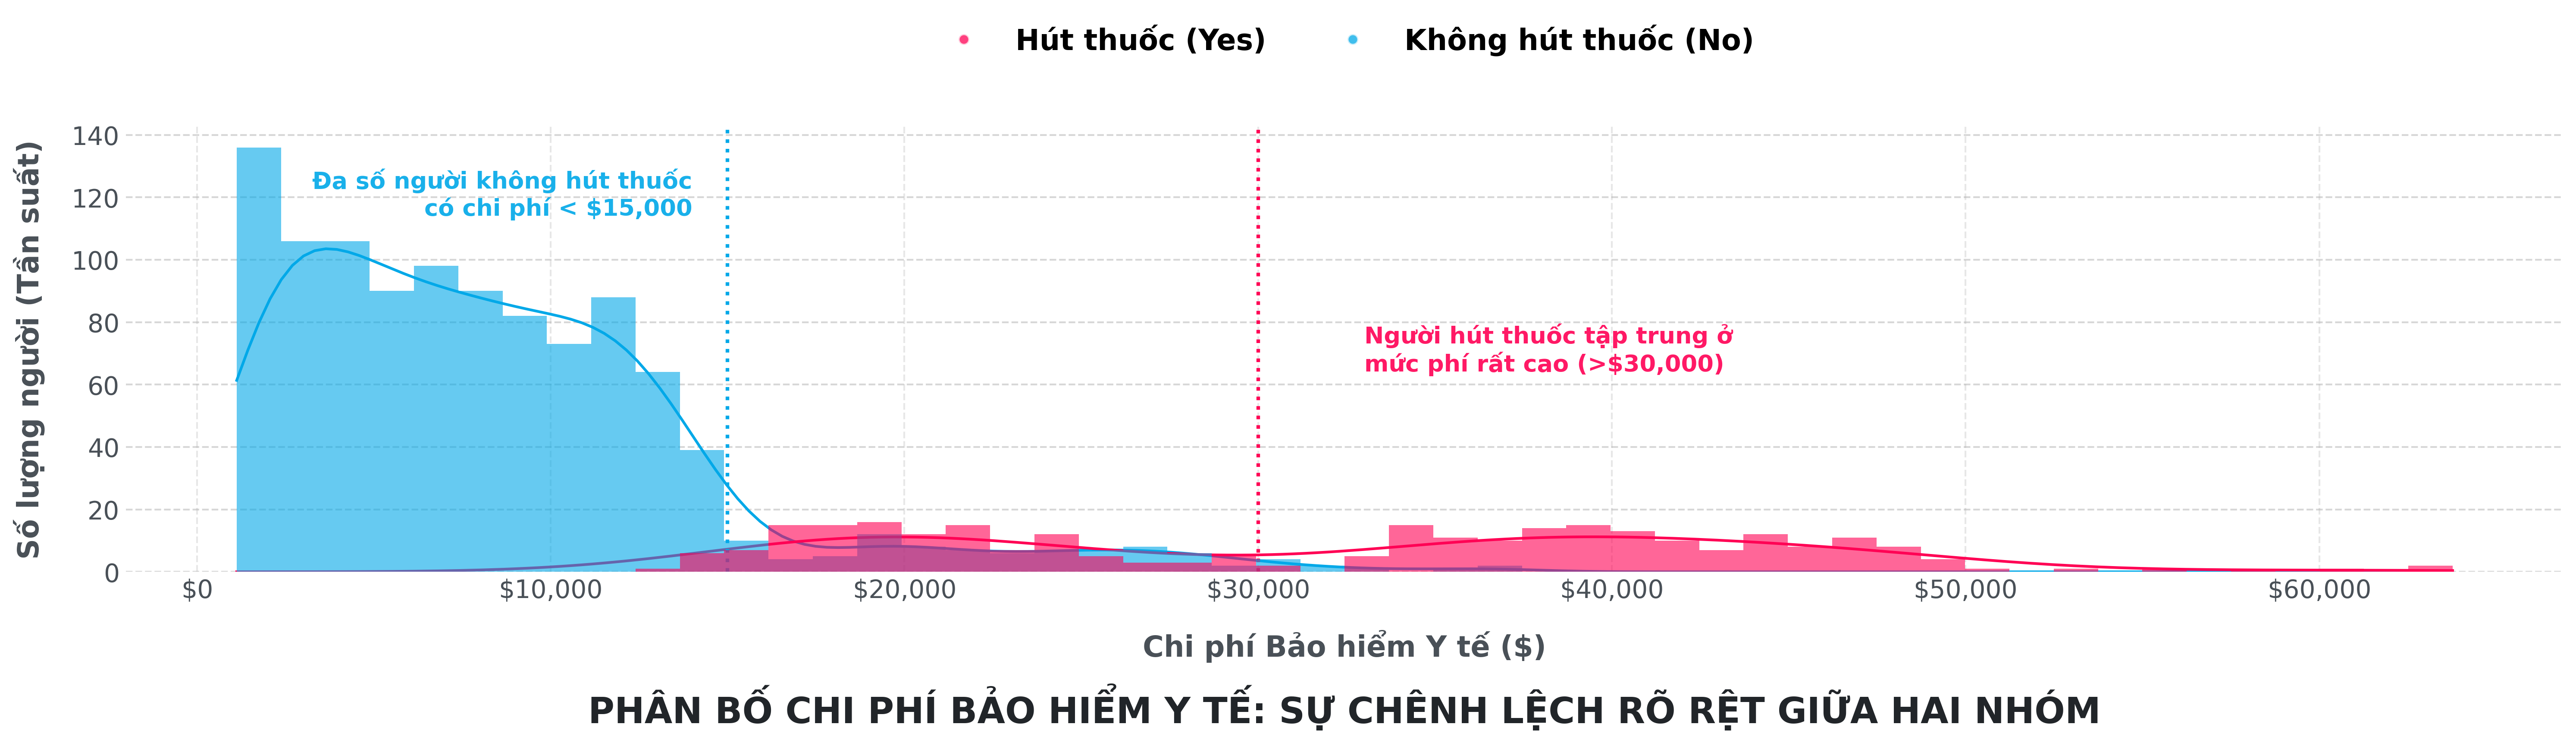
\includegraphics[width=1\linewidth]{images/Medical_Insurance_Dist.png}
    \caption{Phân phối chi phí bảo hiểm y tế (\texttt{charges}). Đuôi dài vắt sang phải cho thấy sự tồn tại của nhóm chi phí ngoại lai rất cao.}
    \label{fig:dist}
\end{figure}

\paragraph{2. Tác động thống kê của thói quen hút thuốc:} 
Biểu đồ Boxplot (Hình \ref{fig:box}) chỉ ra \texttt{smoker} là yếu tố phân loại có discriminative power lớn nhất. Ranh giới IQR giữa hai nhóm gần như không có sự giao thoa. Trung vị chi phí y tế của người hút thuốc rơi vào khoảng trên 30,000 USD, cao gấp nhiều lần nhóm không hút thuốc. Sự tách biệt tuyệt đối này ngụ ý rằng các mô hình Tree-based (như Random Forest hay LightGBM) gần như chắc chắn sẽ ưu tiên chọn biến \texttt{smoker} làm root node trong quá trình phân nhánh không gian đặc trưng.

\begin{figure}[H]
    \centering
    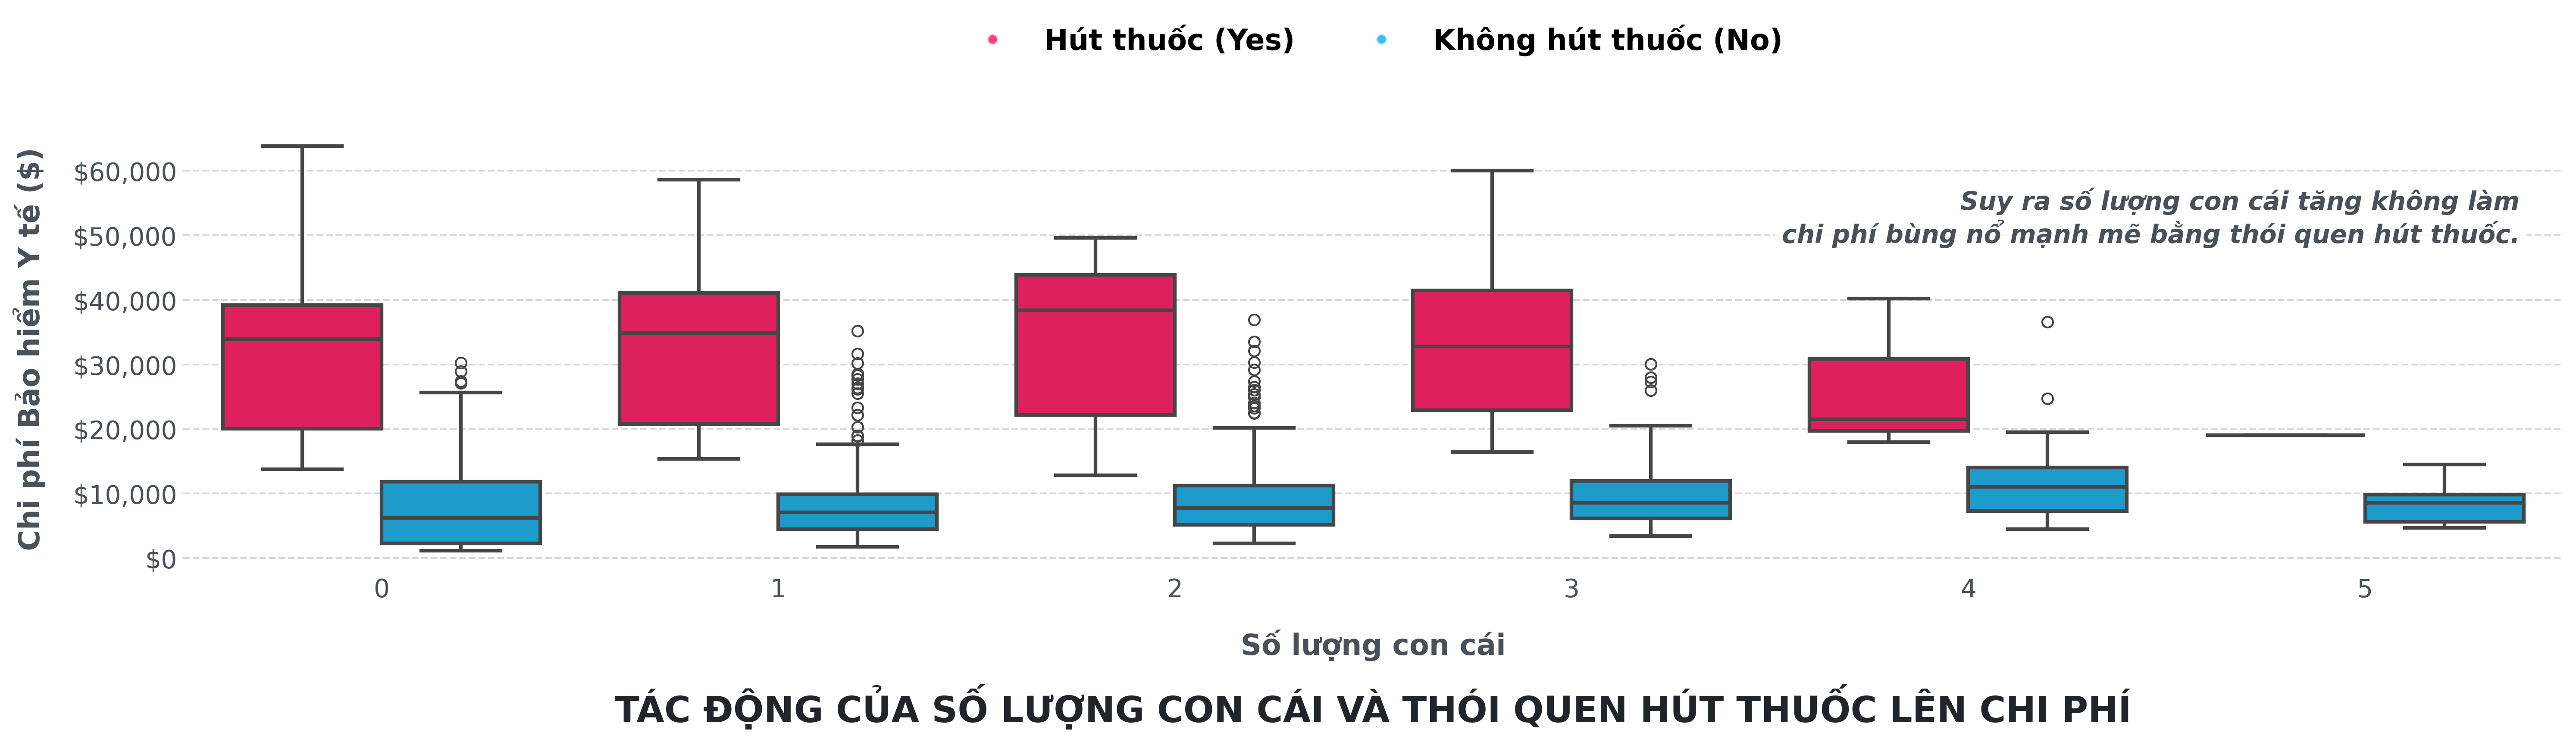
\includegraphics[width=1\linewidth]{images/Medical_Insurance_Box.png}
    \caption{Sự khác biệt về chi phí y tế theo tình trạng hút thuốc thông qua biểu đồ Boxplot.}
    \label{fig:box}
\end{figure}

\paragraph{3. Mối liên hệ phi tuyến giữa BMI, Hút thuốc và Chi phí y tế:}
Biểu đồ phân tán (Hình \ref{fig:scatter_bmi}) biểu diễn một tương tác đa biến cực kỳ thú vị. Nếu chỉ xét riêng \texttt{bmi}, độ tương quan dương với \texttt{charges} là khá yếu. Tuy nhiên, khi lồng ghép thêm yếu tố hút thuốc, dữ liệu bị chẻ làm hai cụm rõ rệt. Đáng chú ý nhất, nhóm khách hàng có BMI > 30 (ngưỡng béo phì) kèm theo thói quen hút thuốc tạo thành một cụm chi phí y tế đột biến. Sự cross-feature interaction mang tính phi tuyến này là nguyên nhân cốt lõi khiến các mô hình tuyến tính truyền thống (Linear Regression) thường thất bại, đồng thời khẳng định sự cần thiết của các mô hình có khả năng học được quy luật phi tuyến phức tạp.

\begin{figure}[H]
    \centering
    
\includegraphics[width=1\linewidth]{images/Medical_Insurance_Scatter.png}
    \caption{Tương quan giữa BMI và chi phí y tế. Cụm điểm tăng vọt phía trên cho thấy hiệu ứng cộng hưởng cực kỳ lớn giữa béo phì và hút thuốc.}
    \label{fig:scatter_bmi}
\end{figure}

\paragraph{4. Tương tác đa biến: Sự hình thành của các dải dữ liệu song song:} 
Khi quan sát chi phí y tế biến thiên theo độ tuổi (Hình \ref{fig:scatter_age}), dữ liệu hội tụ thành 3 dải đường chéo song song. Dải thấp nhất đại diện cho quy luật tự nhiên: chi phí y tế tăng nhẹ và đều đặn theo tuổi tác đối với nhóm người khỏe mạnh (không hút thuốc). Ngược lại, dải cao nhất bị chi phối hoàn toàn bởi nhóm hút thuốc kết hợp với các rủi ro sức khỏe khác. Phân tích này cũng cho thấy yếu tố giới tính (\texttt{sex}) có độ phân tán đồng đều ở cả 3 dải, hàm ý rằng giới tính có thể đóng góp Feature Importance rất thấp trong mô hình cuối cùng.

\begin{figure}[H]
    \centering
    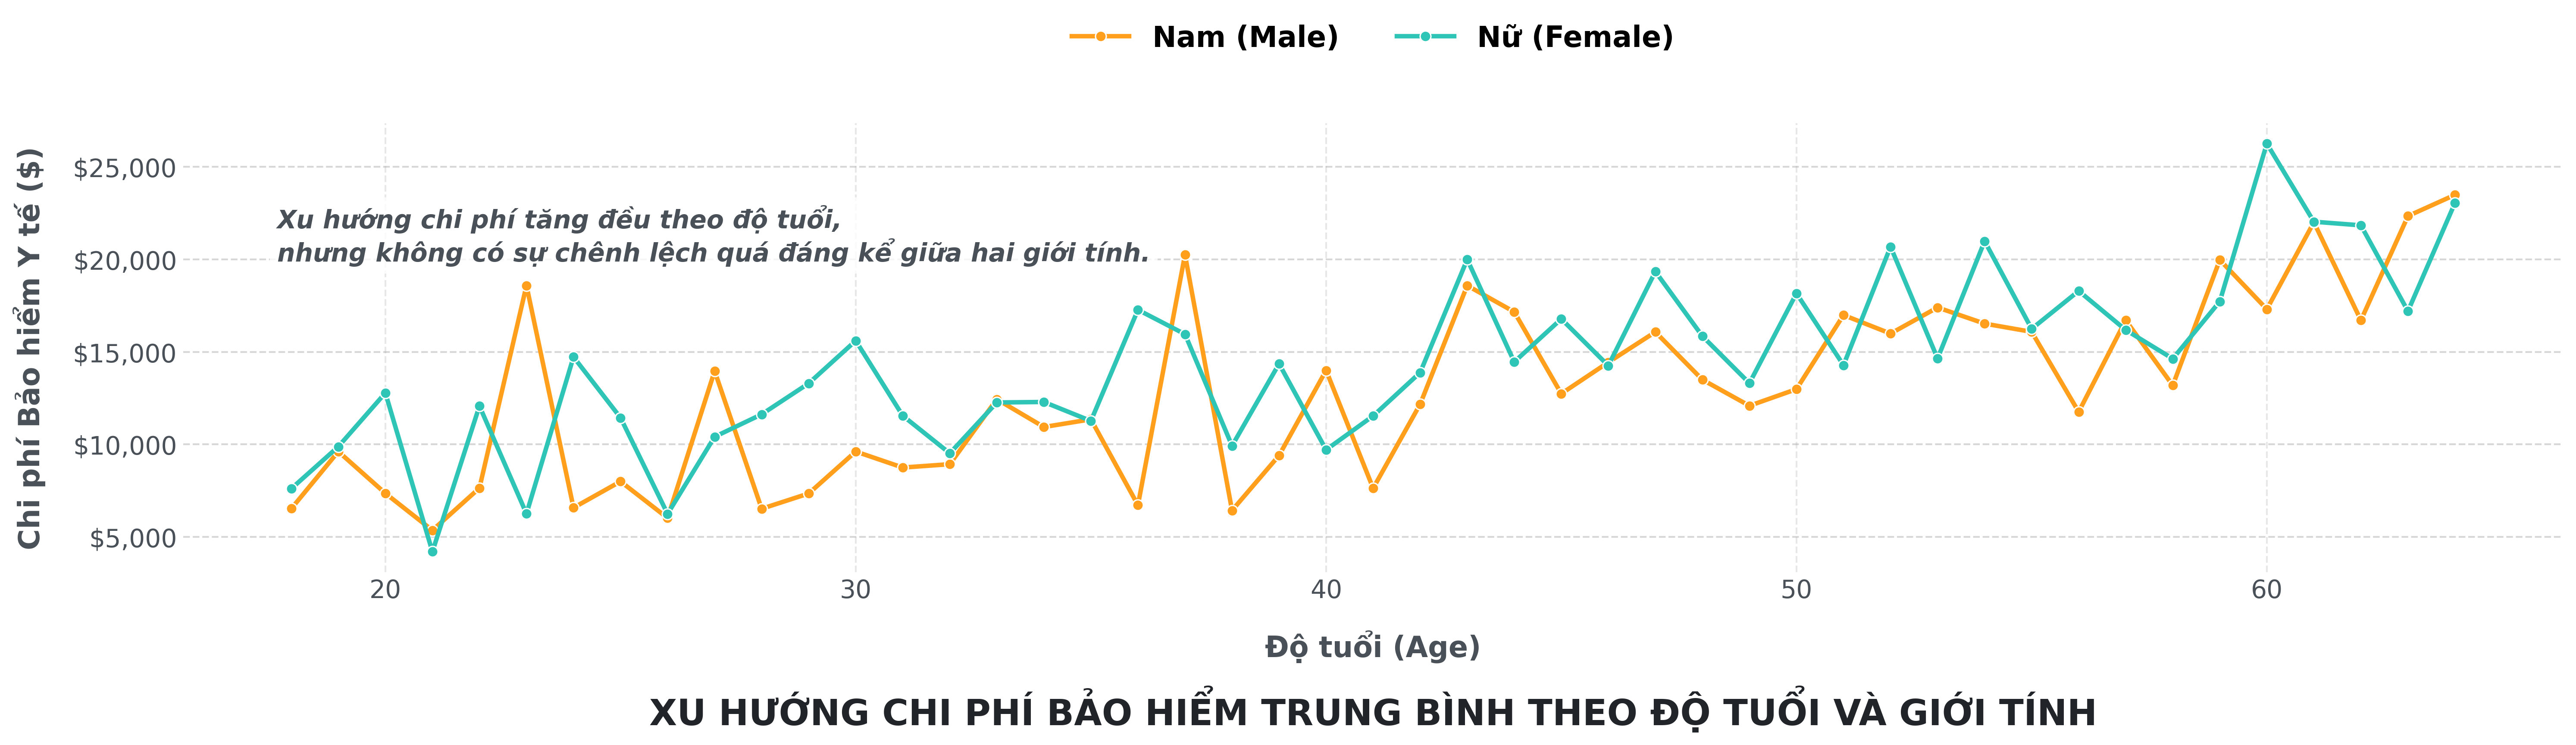
\includegraphics[width=1\linewidth]{images/Medical_Insurance_Age_Sex.png}
    
    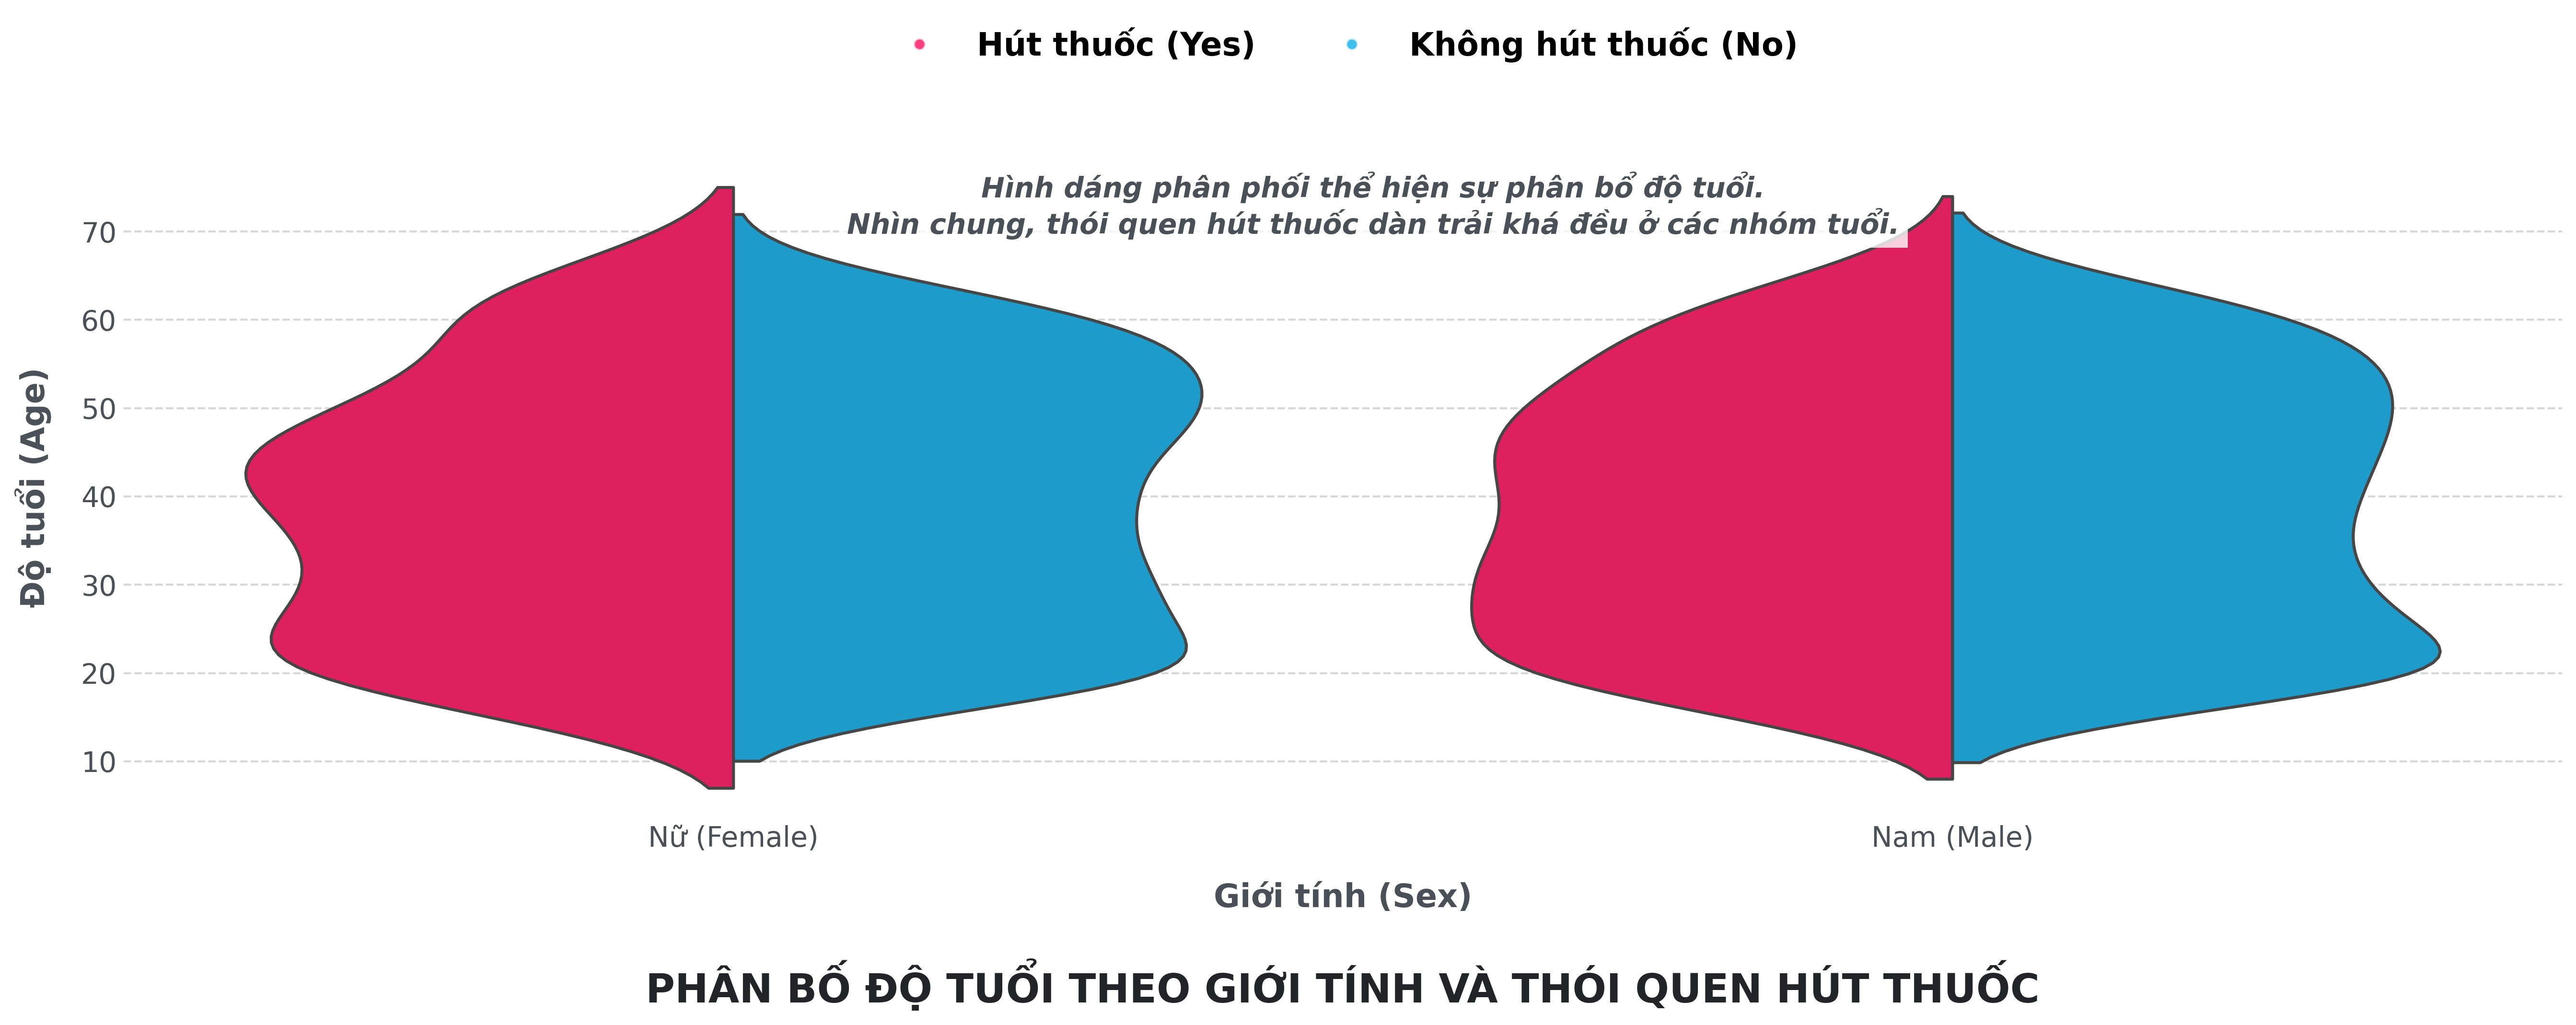
\includegraphics[width=1\linewidth]{images/Medical_Insurance_Age_Sex_Smoker.png}
    \caption{Ba dải dữ liệu song song phân tách theo độ tuổi và tình trạng hút thuốc. Giới tính không tạo ra sự phân biệt rõ ràng.}
    \label{fig:scatter_age}
\end{figure}

\paragraph{5. Tính toàn vẹn và Phân bổ của Categorical Features:}
Biểu đồ Bar chart (Hình \ref{fig:bar}) cung cấp cái nhìn vĩ mô về thiết kế thu thập dữ liệu. Các biến phân loại như khu vực sinh sống (4 vùng tại Mỹ) và giới tính đều có sự phân bổ quan sát xấp xỉ nhau. Sự vắng bóng của hiện tượng Class Imbalance bảo đảm rằng ta không cần phải can thiệp bằng các kỹ thuật resampling (như SMOTE) hay Class Weights. Các mô hình hoàn toàn có thể tự tin học trên dữ liệu nguyên bản mà không lo bị bias về một phân khúc khách hàng đa số nào.

\begin{figure}[H]
    \centering
    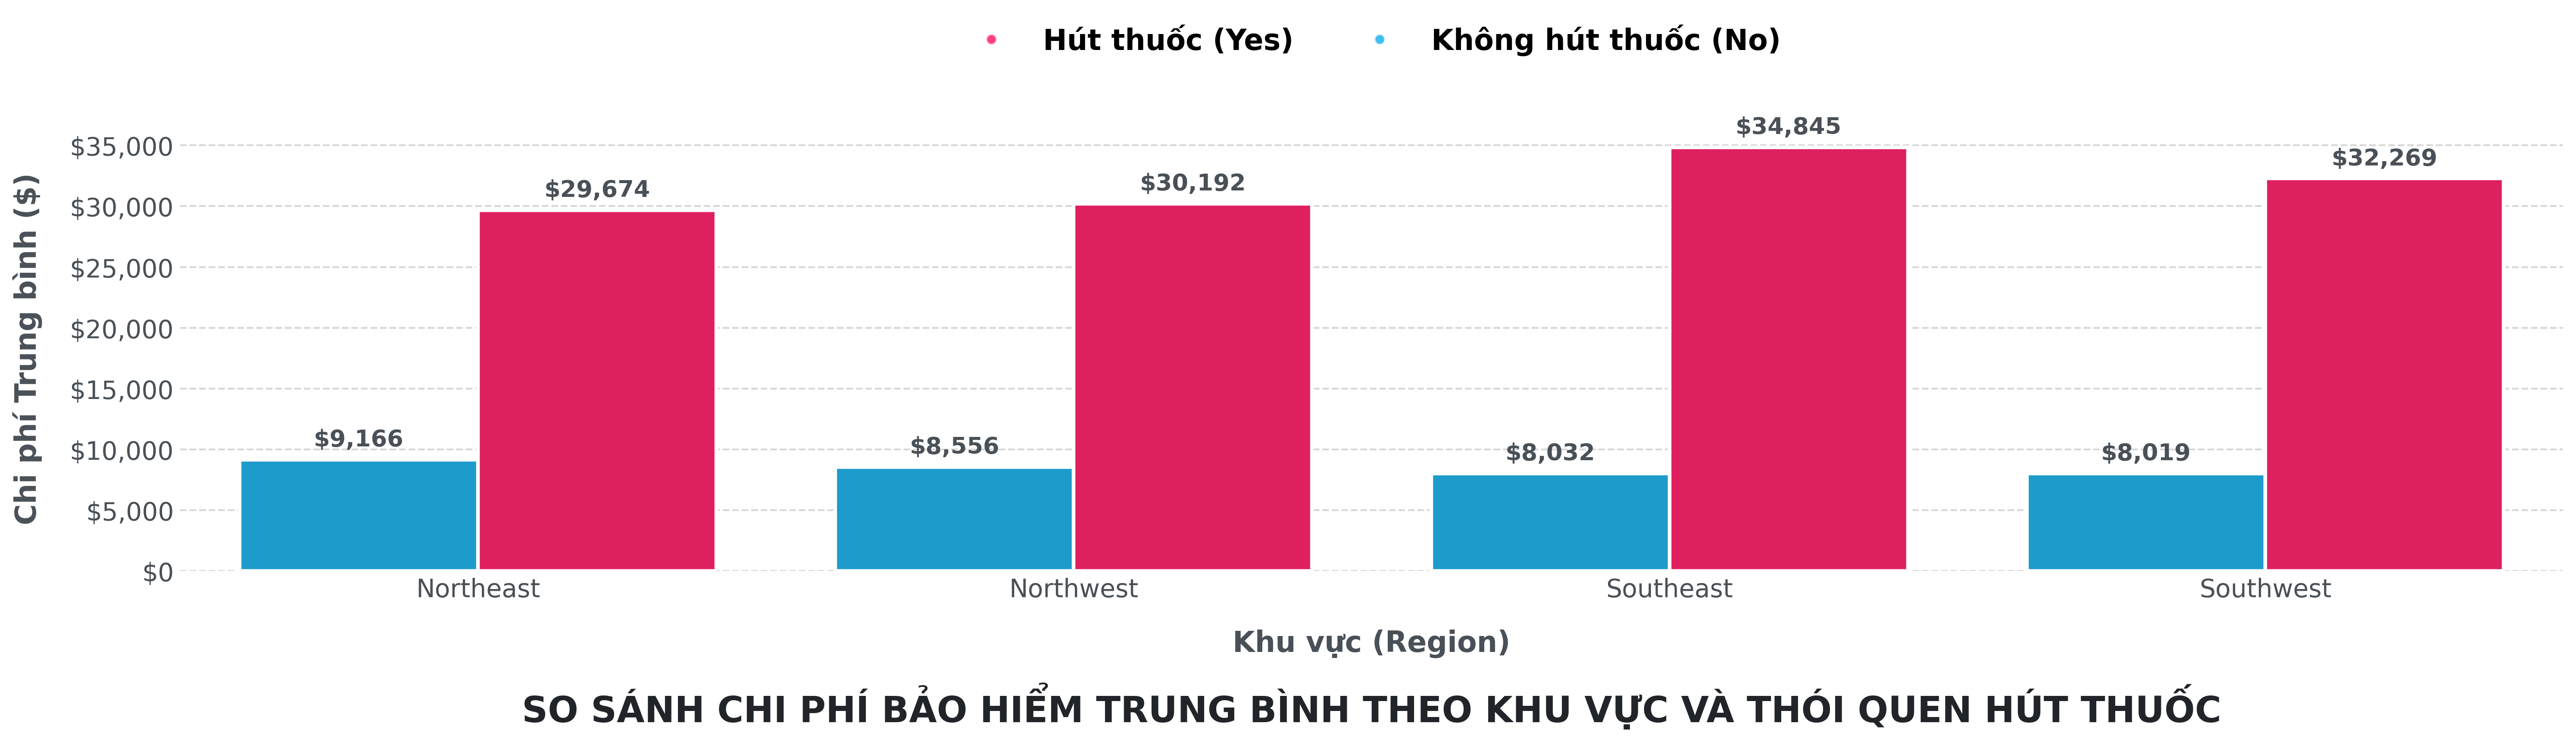
\includegraphics[width=1\linewidth]{images/Medical_Insurance_Bar.png}
    \caption{Phân bố tần suất đồng đều của các biến phân loại, xác nhận không có nhiễu loạn từ hiện tượng Class Imbalance.}
    \label{fig:bar}
\end{figure}
